\section{Inequalities with $\le$ and $<$}

\begin{tcbraster}[
    raster columns = 2,
    raster equal height,
    colback = white,
    ]
    \begin{tcolorbox}
        $|x| \le 3$ 
        \tcblower
        \begin{center}
            \begin{tcolorbox}[center,colback=white,boxrule=0.5pt,]
                \small The distance of $x$ from the origin is \myEmph{less than or equal to} $3$.
            \end{tcolorbox}
            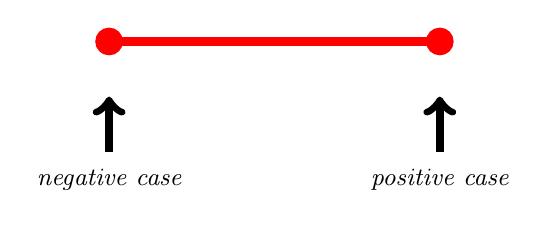
\begin{tikzpicture}[scale=0.7]
                \myDrawNumberlineCircle{0}{white}
                \whenTEACHER{
                    \draw [-,line width=3pt,red] (-3,0) -- (3,0);
                    \draw[red,line width=3pt,fill=red] (-3,0) circle (0.175 cm);
                    \draw[red,line width=3pt,fill=red] (3,0) circle (0.175 cm);
                }
                \draw[->, black, line width=3pt] (-3,-2) -- (-3,-1);
                \node[] at (-3,-2.5) {\itshape\small negative case};
                \draw[->, black, line width=3pt] (3,-2)  -- (3,-1);
                \node[] at (3,-2.5) {\itshape\small positive case};
                \myDrawNumberline{5}
            \end{tikzpicture}\\
            \whenSTUDENT{\vspace{2\onelineskip}}
            %
            \whenTEACHER{
                {
                    $-3 \le x \le 3$
                }
            }
            \end{center}
    \end{tcolorbox}
    \begin{tcolorbox}
        $|x| < 3$ 
        \tcblower
        \begin{center}
            \begin{tcolorbox}[center,colback=white,boxrule=0.5pt,]
                \small The distance of $x$ from the origin is \myEmph{less than} $3$.
            \end{tcolorbox}
            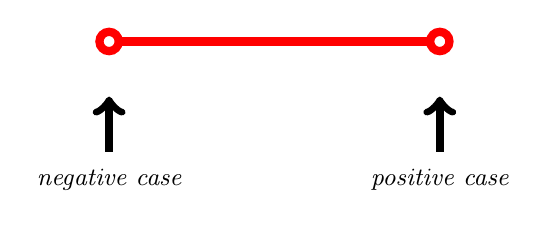
\begin{tikzpicture}[scale=0.7]
                \myDrawNumberlineCircle{0}{white}
                \whenTEACHER{
                    \draw [-,line width=3pt,red] (-3,0) -- (3,0);
                    \draw[red,line width=3pt,fill=white] (-3,0) circle (0.175 cm);
                    \draw[red,line width=3pt,fill=white] (3,0) circle (0.175 cm);
                }
                \draw[->, black, line width=3pt] (-3,-2) -- (-3,-1);
                \node[] at (-3,-2.5) {\itshape\small negative case};
                \draw[->, black, line width=3pt] (3,-2)  -- (3,-1);
                \node[] at (3,-2.5) {\itshape\small positive case};
                \myDrawNumberline{5}
            \end{tikzpicture}\\
            \whenSTUDENT{\vspace{2\onelineskip}}
            %
            \whenTEACHER{
                {
                    $-3 < x < 3$
                }
            }
            \end{center}
    \end{tcolorbox}
\end{tcbraster}


\begin{myConceptSteps}{To solve $|ax+b|\le c$ or $|ax+b| < c$\dots}
    \myStep{check}{Be careful if $c$ is \gap{zero} or \gap{negative}.\\
        \vspace{-1.25\onelineskip}
        \begin{center}
        \begin{tabular}{|l|c|}
            \hline
            $|ax+b| <$ \myEmph{negative} & \gap{no} \gap{solution} \\
            \hline
            $|ax+b| <$ \myEmph{zero}     & \gap{no} \gap{solution} \\
            \hline
            $|ax+b| \le$ \myEmph{zero}   & only solve \gap{$= 0$}  \\
            \hline
        \end{tabular}
        \end{center}
    }
    \myStep{three-part inequality}{Write a three part inequality: 
        \begin{itemize}[nosep]
            \item 
                $ -c $
                \gap{$\le \text{or} <$}
                $| ax+b |$
                \gap{$\le \text{or} <$}
                $ c $
        \end{itemize}
    }
    \myStep{solve}{
        Solve the inequality, getting the variable in the \gap{middle} by itself.
        \begin{myWarningBox}[width=5.5in,center]
            \small\centering
            \gap{Multiplying}/\gap{dividing} by negatives \gap{flips} the inequality.
        \end{myWarningBox}
    }
    \myStep{result}{Write the result in two ways.
        \begin{itemize}[nosep]
            \item as as a 3-part inequality with the variable in the middle
            \item an interval on the number line
        \end{itemize}
    }
\end{myConceptSteps}

\myProblems[Solve these absolute value inequalities.]
{
    $|21-3x| \le 9$
    \myAnswer{
        \hfill
        {\tiny 
            $4 \le x \le 10$
        }
    }
}
{
    $|4 - \frac{3}{4}x| < 5$
    \myAnswer{
        \hfill
        {\tiny 
            $-\frac{4}{3} < x < 12$
        }
    }
}
{10\onelineskip}